% file: kap_zakld_zakn_elmag.tex
%====================Kapitola: Základní zákony elektromagnetismu====================================
\chapter{Základní zákony elektromagnetismu}\label{ES:kap_zaklzelmg}
\minitoc
\newpage
  \section{Magnetická indukce}
    V této teoreticky změřené kapitole budou shrnuty základní fyzikální zákony, kterými se řídí
    elektromagnetické jevy a jejichž znalost bude nezbytná při studiu následujících praktičtěji
    zaměřených kapitol. Mizi nejdůležitější patří zákon elektromagnetické indukce. Velký praktický
    váznam má jeho zobecnění i pro případy nejsložitějsí, jakými jsou \emph{nelineární} a navíc
    \emph{parametrické} magnetické obody. Důležitým pojmem je \emph{spřažený} magnetický tok cívky.
    Pro hlubší pochopení všech zákonitostí bude vhodné upozornit na \emph{topologické vlatnosti}
    elektromagnetického pole. Ukazuje se totiž, že topologický přístup je velice užitečným a silným
    nástrojem, který významně usnadňuje pochopení
    \href{http://en.wikipedia.org/wiki/Maxwell_theory}{Maxwellových rovnic} se všemi jejich důsledky
    \cite[s.~6]{Patocka4}. Topologii elektromagnetického pole je proto věnována celá kapitola
    \ref{ES:kap_topovlelmagp}

    \begin{figure}{r}
      \centering
      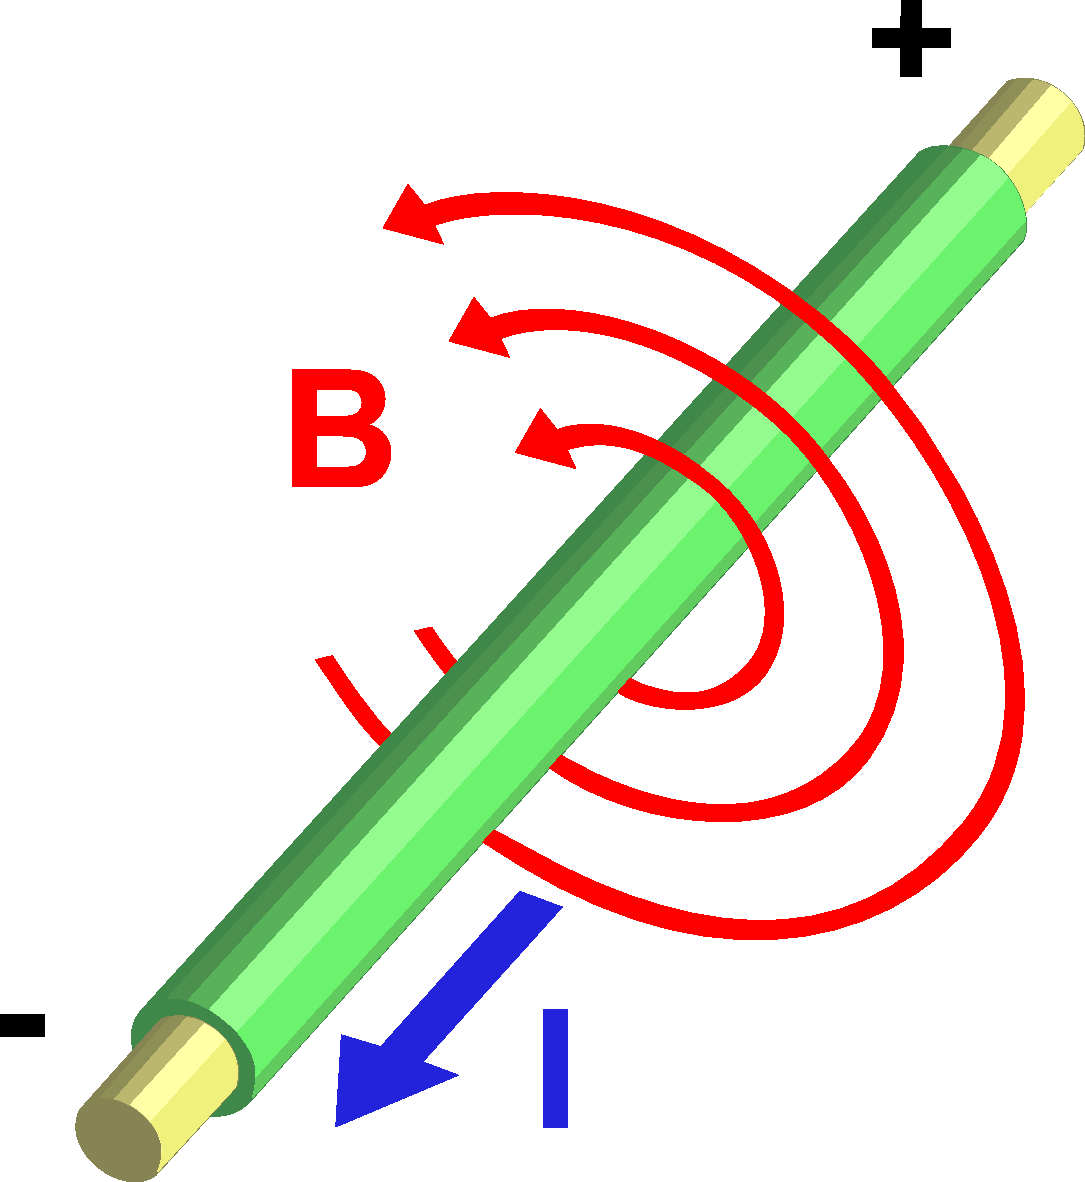
\includegraphics[width=0.5\linewidth]{Amperes_circuital_law.pdf}
      \caption{Elektrický proud ve vodiči způsobuje vznik magnetické pole v jeho okolí.}
      \label{ES:fig_amp_law}
    \end{figure}   
    Základní veličinou pro popis magnetických polí a jejich účinků je \emph{vektor magnetické
    indukce} - \(\vec{B}\). Dle soustavy SI je jednotkou magnetické indukce \emph{tesla} \([T]\) a
    projevuje se silovými účinky na vodiče protékané proudy a indukováním napětí při jeho změně.

    Je proto dobře měřitelný. První rovnice (Ampérův zákon) ze souboru Maxwellových rovnic určuje
    rovnost oběhového integrálu magnetické indukce po uzavřené křivce proudům protékaných vodiči,
    jež jsou touto křivkou uzavřeny.
    \begin{equation}\label{es:eq_amp_law}
      \oint_l \vr{B} \cdot d\vr{l} = \sum I
    \end{equation}
    $\mu_0 = 4\pi\cdot 10^{-7}$ 
    H/m je magnetická konstanta - \textbf{permeabilita vakua}. Elektrické proudy jsou stále
    obklopeny magnetickými poli. Tato pole se dají zesílit cívkou s magnetickým jádrem. Na tomto
    jevu je založen jeden z elementárních principů elektrotechniky.
    
    Protože je tento zákon stěžejní k pochopení ostatních principů, je vhodné si také uvědomit
    vztah jednotky magnetické indukce k základním jednotkám soustavy \textbf{SI}: $$1T =
    1\frac{V\cdot s}{m^2} = 1\frac{N}{A\cdot m} = 1\frac{Wb}{m^2} = 1\frac{kg}{C\cdot s} =
    1\frac{kg}{A\cdot s^2} = 1\frac{N\cdot s}{C \cdot m}$$
      
  \section{Zákon elektromagnetické indukce}
    Základní laboratorní experimenty, vedoucí k odhalení existence elektromagnetické indukce,
    uskutečnil \emph{Faraday}\footnote{Michael Faraday (1791 - 1867), samouk, zakladatel klasické
    elektrodynamiky, vynikající experimentátor: Zavedl pojem fyzikálního prostorového pole pomocí
    siločar, tzv. ''trubic''} r. 1831.
    Matematickou formulaci \emph{indukčního zákona} v podobě rovnice
    \begin{equation}
      u(t) = - \frac{d\Psi(t)}{dt}
    \end{equation} 
    stanovil již on sám, postupně význam zákona formálně upřesňovali další badatelé např.
    \emph{Neumann}\footnote{Franz Ernst Neumann (1798 - 1895), teoretický fyzik, matematik,
    mineralog. Definoval pojem magnetický vektorový potenciál, formuloval Neumannův vzorec pro
    vzájemnou indukčnost dvou smyček. Učitel G. R. Kirchhoffa.} kolem roku 1845. Konečné znění
    Maxwellovy teorie včetně formulace indukčního zákona do podoby II. Maxwellovy rovnice budoval
    Maxwell\footnote{James Clark Maxwell (1831 - 1879), teoretický fyzik, působil na Trinity
    College university v Cambridge, na King's College v Londýně, posléze první ředitel Cavendishovy
    laboratoře na univerzitě v Cambridge. Původně se zabýval teoretickou mechanikou a kinetickou
    teorií plynů. Soustavu čtyř Maxwellových rovnic odvodil především na základě
    mechanicko-elektrických analogií.} velmi pozvolna, v období 1855 až 1873. Z historického pohledu
    je zajímavé a důležité, ře přesné \emph{kvantitativní} experimenty s elektromagnetickou indukcí
    byly v té době uskutečnitelné pouze pomocí
    \href{http://en.wikipedia.org/wiki/Galvanometer}{balistického galvanoměru}. Lze odhadnout, že
    nebýt tohoto přístroje, přesná matematická formulace indukčního zákona by se praděpodobně
    opozdila o několik let. Kupodivu, z psychologického hlediska je i v současnosti velmi vhodné
    vysvětlit princip indukčního zákona pomocí historických pokusů s balistickým galvanoměrem.
    
    Jako každý elektromagnetický měnič energie (tj. motor), obsahuje i \emph{magnetoelektrické
    měřicí} ústrojí galvanoměru dva akumulátory energie: moment setrvačnosti \(J\) otoč\-né části a
    indukčnost cívky \(L\). Jedná se tedy o kmitavou soustavu 2. řádu. Každou takovou soustavu lze
    kriticky, případně nadkriticky tlumit - především zařazením tlumicího odporu vhodné velikosti do
    série s měřicím systémem (tlumení vlivem mechanického třejí je úmyslně konstrukčně potlačeno na
    zanedbatelnou úroveň). Balistický galvanoměr je cíleně konstruován s velkým momentem
    setrvačnosti \(J\) a s malou tuhostí \(k_d\) direkčních pružin, aby měl dlouhou dobu kmitu \(T_G
    = 2\pi\sqrt{J/k_d}\) několik sekund. Proteče-li galvanoměrem krátký proudoý impuls \(i(t)\) o
    celkové délce \(t_i\) podle obr. \ref{ES:fig_imp_glvn}, pak lze snadno dokázat, že za
    předpokladu \(t_i\ll T_G\) je první maximální výchylka \(\alpha_{max}\) tlumeného pohybu
    ukazatele přímo úměrná celkovému náboji \(Q\) proudového impulsu podle rovnice 
    \begin{equation}\label{ES:eq_zakl_elm01}
      \alpha_{max} = k_b Q = k_b\int_0^{t_i} i(t)dt,
    \end{equation}
    kde \(k_b\) je \emph{balistická konstanta} použitého galvanoměru. Balistický galvanoměr tedy
    pracuje jako \emph{integrátor} proudu v přesném matematickém smyslu. 

    %----------------------------------
    % image: patocka_balist_glvn.tex label: \label{ES:fig_imp_glvn}
      %\documentclass{book}
%\usepackage{tikz}
%\usepackage{pstricks}
%  \usetikzlibrary{intersections}
%  \usetikzlibrary{calc}

%\newpath
%\moveto(0.37880683,-0.12631738)
%\curveto(0.37880683,-0.12631738)(16.746964,-0.16331738)(27.401489,14.35218262)
%\curveto(38.204079,29.06968262)(51.661079,58.47632262)(63.387069,58.58885262)
%\curveto(75.113069,58.70138262)(81.146179,32.79738262)(97.499259,19.26928262)
%\curveto(116.61771,3.45338262)(143.05509,-0.35661738)(143.05509,-0.35661738)
   
%\begin{document}
\begin{figure}[ht!]
  \centering
  \begin{tikzpicture}
	\def\xmin{0}
	\def\xmax{160}
	\def\ymin{-3}
	\def\ymax{80}
	\def\nula{0}
	\def\phase{0}
		
		\begin{scope}[draw=black,line join=round,miter limit=4.00,line width=0.5pt, y=1pt,x=1pt]
		  \draw[->] (\xmin,\nula) -- (\xmax,\nula) node[right] {$t$} coordinate(x axis);
		  \draw[->] (\phase,\ymin) -- (\phase,\ymax) node[left]  {$i(t)$} coordinate(y axis);
		  \path[name path=fce,draw=black,line join=round,even odd rule,line cap=butt,miter
			limit=4.00] (0,0)             .. controls
           (0,0)   and (17,0)  .. (27,14) .. controls
           (38,29) and (52,58) .. (63,58) .. controls
           (75,58) and (81,33) .. (97,19) .. controls
           (117,3) and (143,0) .. (143,0);			
			
		  \path[name path=osax] (\xmin,\nula) -- (\xmax,\nula);
		  
	      % Intersections
          \path[name intersections={of=osax and fce, name=point}];   % prusecik osy x s funkc�
          \draw[name path=line1] (point-1) ++ (0,-2) node[below] {$0$};
		  \draw[name path=line1] (point-2) ++ (0,-2) node[below] {$t_i$}  --+(0,4);
		  \node[left]  at (70,25) {$Q$};         		 
		\end{scope}		
  \end{tikzpicture} 
  \caption{Příklad krátkého proudového impulsu prošlého balistickým
           galvanoměrem.}\label{ES:fig_imp_glvn}
\end{figure}  
%\end{document}
  
    %----------------------------------    
    
    Uvažujme experiment uspořádaný podle obr. \ref{es:fig_MJ_patocka_glvnmr}. V uzavřeném obvodu
    galvanoměru se nachází celkový odpor \(R\) a tuhá samonosná cívka v podobě kruhového závitu,
    připojená na dlouhé ohebné zkroucené přívody. Husté zkroucení zajišťuje, že do samotných
    přívodů se nemůže indukovat žádné napětí, pohybuje-li se cívka v magnetickém poli permanentního
    magnetu. Při rychlém přesunu z polohy \emph{I} do vzdálené polohy \(\infty\) klesne v cívce
    magnetický tok na nulu, časová změna toku zapříčiní vznik indukovaného napětí, napětí protlačí
    obvodem proudový impuls odpovídající přibližně obr. \ref{ES:fig_imp_glvn}.

    \begin{figure}[ht!]
      \centering
      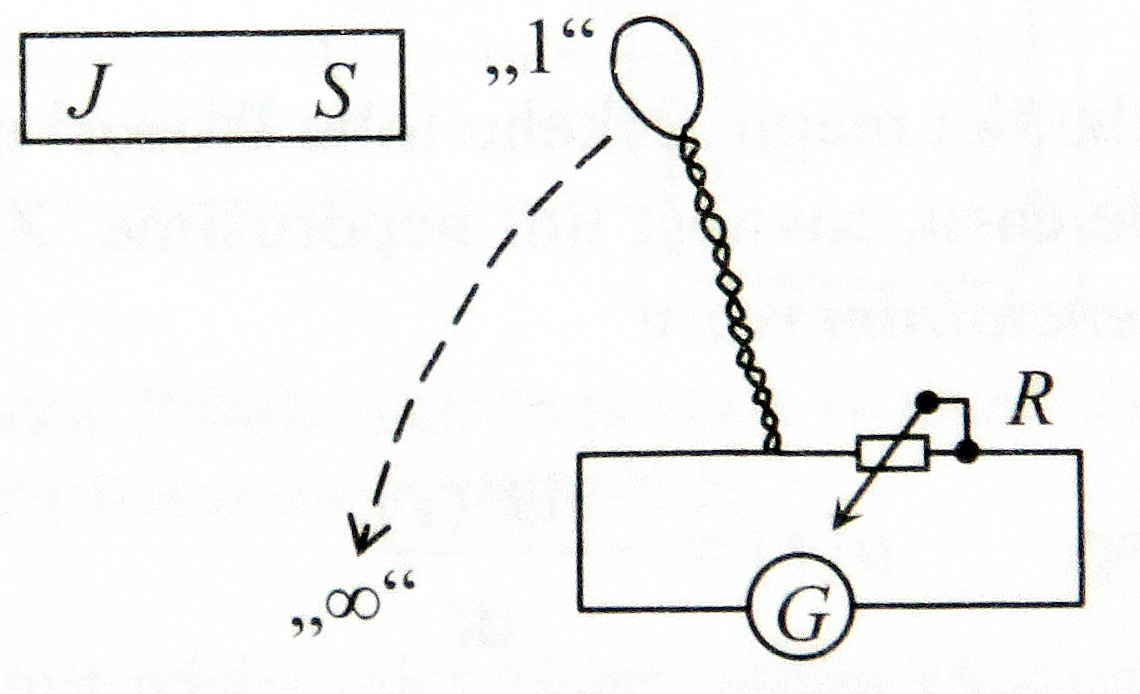
\includegraphics[width=0.9\linewidth]{MJ_patocka_glvnmr.JPG}
      \caption[Uspořádání experimentálního pracovište s balistickým galvanoměrem.]{Uspořádání
               experimentálního pracovište s balistickým galvanoměrem}
      \label{es:fig_MJ_patocka_glvnmr}
    \end{figure}   
    Za předpokladu kritického nebo nadkritického tlumení má odpor \(R\) relativně velkou hodnotu. Proto lze s 
    dobrou přesností zanedbat vnitřní indukčnost měřicího systému galvanoměru a uvažovat, že celé napětí 
    \(u(t)\), indukované v cívce při jejím pohybu, spočine pouze na odporu. V uzavřeném okruhu o celkovém 
    odporu \(R\) pak platí Ohmův zákon ve tvaru
    \begin{equation}\label{ES:eq_zakl_elm02}
      i(t)=\frac{u(t)}{R}.
    \end{equation}    
    Dosadíme-li rovnici \ref{ES:eq_zakl_elm02} do \ref{ES:eq_zakl_elm01}, po úpravě získáme vztah
    \begin{equation}\label{ES:eq_zakl_elm03}
     \int_0^{t_i}u(t)dt=\frac{\alpha_{max}R}{k_b}.
    \end{equation}     
    Experimentálně je možno dospět ke dvěma stěžejním poznatkům:
    \begin{itemize}
      \item Při přesunu cívky z polohy \emph{I} do polohy \(\infty\) nezávisí výchylka
            \(\alpha_{max}\) na \emph{rychlosti pohybu}. (Za předpokladu \(t_i\ll T_G\), což je
            omezení dané nedokonalostí přístroje a nijak nesouvisí se zkoumaným jevem.)
      \item Při přesunu cívky z polohy \emph{I} do polohy \(\infty\) zůstává součin
            (\(\alpha_{max}\times R\)) stále \emph{konstantní}, měníme-li úmyslně velikost odporu
            \(R\). To jest: při k-násobném zvýšení odporu klesne výchlka k-krát a naopak. 
    \end{itemize}

    V poloze „1“ prochází plochou cívky magnetický tok \(\Psi\). V poloze „\(\infty\)“ je zřejmě
    magnetický tok cívky nulový, tedy \(\Psi_\infty = 0\). S ohledem na rovnici
    (\ref{ES:eq_zakl_elm03}) lze pak oba experimentální poznatky interpretovat jediným možným
    způsobem:
     \begin{equation}\label{ES:eq_zakl_elm04}
     \int_0^{t_i}u(t)dt=\text{konst}=\Psi-\Psi_\infty=\Psi.
    \end{equation}    

    Experiment lze opakovat s cívkami libovolných rozměrů, tvarů i počtů závitů. Výsledky budou
    kvalitativně stejné. Veličina \(\Psi\) se nazývá \emph{spředený magnetický tok cívky}. Je to
    míra interakce cívky s magnetickým polem, které spojitě prostupuje celou plochou cívky. Rovnici
    (\ref{ES:eq_zakl_elm04}) lze vyjádřit slovně: Spřažený magnetický tok cívky je úměrný časovému
    integrálu svorkového napětí na zkoumané cívce. Je určitě výhodné zvolit jedničku jako konstantu
    úměrnosti mezi tokem \(\Psi\) a integrálem napětí. \emph{Pak bude velikost spřaženého toku přímo
    rovna integrálu napětí}. Určitý integrál v rovnici (\ref{ES:eq_zakl_elm04}) lze nahradit
    integrálem neurčitým, pak je ale nutno přidat obecnou počáteční integrační konstantu \(\Psi_0\)
    v newtonovském smyslu. Získáme tak zákon elektromagnetické indukce (indukční zákon) v
    integrálním tvaru
    \begin{equation}\label{ES:eq_zakl_elm05}
     \Psi(t) = \Psi_0 + \int u(t)dt \quad [Wb;\, V,\; s].
    \end{equation}   
    
    Z rovnice (\ref{ES:eq_zakl_elm05}) plyne, že jednotka magnetického toku Weber\footnote{Wilhelm
    Eduard Weber (1804-1891), teoretický fyzik, působil na univerzitách v Gottingenu a v Lipsku.
    Zakladatel předrelativistické elektrodynamiky. Určil totiž silu mezi náboji v závislosti nejen
    na vzdálenosti, ale i na rychlosti a zrychlení, jeho teorie je ale platná pouze pro \(v \ll c\).
    Blízký spolupracovník Gausse.} má rozměr \([Vs]\), Budeme-li obě strany rovnice derivovat podle
    času, rovnost tím neporušíme. Získáme tak ryze matematickou cestou indukční zákon v
    diferenciálním tvaru
    \begin{equation}\label{ES:eq_zakl_elm06}
     u(t) = \frac{d\Psi(t)}{dt}, \qquad \text{resp.} \qquad  u(t) = -\frac{d\Psi(t)}{dt}.
    \end{equation}   
    Obě rovnice (\ref{ES:eq_zakl_elm06}a), (\ref{ES:eq_zakl_elm06}b) se liší znaménkem \(+\) nebo
    \(-\) na pravé straně. Volba znaménka souvisí s domluvou, který režim cívky považujeme za
    základní: zda režim \emph{spotřebičový} podle rovnice (\ref{ES:eq_zakl_elm06}a), nebo režim
    \emph{zdrojový} podle rovnice (\ref{ES:eq_zakl_elm06}b). Oba režimy jakéhokoli dvojpólu jsou
    totiž jednoznačně definovány vzájemnou orientací napětí a proudu podle obr.
    \ref{es:fig_MJ_patocka_spbzdr}. Odpor nemůže nikdy pracovat jako zdroj, proto slouží jako
    „normál“ definující \emph{spotřebičovou} orientaci svorkových veličin. Oba režimy cívky se liší
    níže popsaným způsobem.

%     \begin{figure}[ht!]
%       \centering
%       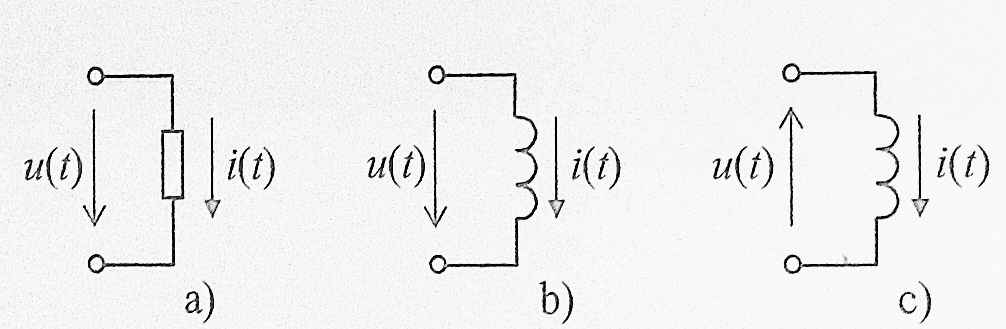
\includegraphics[width=0.5\textwidth]{MJ_patocka_ind.JPG}
%       \caption[Vzájemná orientace okamžité hodnoty proudu a napětí ve spotřebičovém a
%                zdrojovém režimu.]{Vzájemná orientace okamžité hodnoty proudu a napětí ve
%                spotřebičovém a zdrojovém režimu. a) Odpor je vždy spotřebičem. b) Cívka ve
%                spotřebičovém režimu. c) Cívka ve zdrojovém režimu.}
%       \label{es:fig_MJ_patocka_spbzdr}
%     \end{figure}
    %----------------------------------
    % image: MJ_patocka_spbzdr.tex label: \label{es:fig_MJ_patocka_spbzdr}
      % \documentclass{article}
%   \usepackage{circuitikz}  
%   \usepackage{tikz}
%     \usetikzlibrary{decorations.markings}
% 	\usetikzlibrary{arrows.new}  
%   \usepackage{wrapfig}
%   \usepackage{subfig}
%   
% \begin{document}
  \begin{figure}[htp]
    \centering
    \subfloat[ ]   {
        \begin{circuitikz}[scale=1, every node/.style={scale=1}]
          \draw (0,0) node[ocirc] {} --+ (1,0) coordinate(A); 
          \coordinate (B) at ([yshift=-2.5cm]A);
          \draw (A) to[R] (B) --+ (-1,0) coordinate(D) node[ocirc] {}; 
		  
		  \begin{scope}[shorten >= 10pt,shorten <= 10pt]
		  
            \draw[-open triangle 45 new,arrow head=5pt]
			     ([xshift=.6cm,yshift=-0.5cm]A) -- node[right] {$i(t)$} 
			     ([xshift=.6cm,yshift=0.5cm]B); 
	        \draw[->]  (0,0) -- node[left] {$u(t)$} (D);			
	      \end{scope}		  
        \end{circuitikz}    
    }
    \subfloat[ ]   {
        \begin{circuitikz}[scale=1, every node/.style={scale=1}]
          \draw (0,0) node[ocirc] {} --+ (1,0) coordinate(A); 
          \coordinate (B) at ([yshift=-2.5cm]A);
          \draw (A) to[L] (B) --+ (-1,0) coordinate(D) node[ocirc] {}; 
	      
		  \begin{scope}[shorten >= 10pt,shorten <= 10pt]
	        \draw[-open triangle 45 new,arrow head=5pt] 
  			     ([xshift=.6cm,yshift=-0.5cm]A) -- node[right] {$i(t)$} 
  			     ([xshift=.6cm,yshift=0.5cm]B); 
	        \draw[->]  (0,0) -- node[left] {$u(t)$} (D);
	      \end{scope}		  
        \end{circuitikz}
    }  
    \subfloat[ ]   {
        \begin{circuitikz}[scale=1, every node/.style={scale=1}]
          \draw (0,0) node[ocirc] {} --+ (1,0) coordinate(A); 
          \coordinate (B) at ([yshift=-2.5cm]A);
          \draw (A) to[L] (B) --+ (-1,0) coordinate(D) node[ocirc] {}; 
	      
		  \begin{scope}[shorten >= 10pt,shorten <= 10pt]
	        \draw[open triangle 45 new-,arrow head=5pt]  
			     ([xshift=.6cm,yshift=-0.5cm]A) -- node[right] {$i(t)$} 
			     ([xshift=.6cm,yshift=0.5cm]B); 
	        \draw[->]  (0,0) -- node[left] {$u(t)$} (D);
	      \end{scope}		  
        \end{circuitikz}
    } 	 

	\caption{Vzájemná orientace okamžité hodnoty proudu a napětí ve spotřebičovém a
             zdrojovém režimu: a) Odpor je vždy spotřebičem. b) Cívka ve spotřebičovém režimu. 
             c) Cívka ve zdrojovém režimu.}
    \label{es:fig_MJ_patocka_spbzdr}
  \end{figure} 
% \end{document}   
    %----------------------------------
        
    \textbf{Spotřebičový režim:}
    \begin{itemize}
      \item Orientace svorkového napětí \(u(t)\) je vůči proudu \(i(t)\) souhlasná. Platí rovnice
            (\ref{ES:eq_zakl_elm06}a).
      \item Cívka je připojena na zdroj napětí\( u(t)\), odebírá z něj proud \(i(t)\), tedy odebírá
            ze zdroje elektrickou energii a chová se jako spotřebič. Tuto energii přeměňuje na
            energii magnetického pole.
      \item Mezi směrem proudu a směrem toku platí \emph{pravidlo pravé ruky}, PPR.           
    \end{itemize}
    
    \textbf{Zdrojový režim:}
    \begin{itemize}
      \item Orientace svorkového napětí u(t) je vůči proudu i(t) nesouhlasná. Platí rovnice
            (\ref{ES:eq_zakl_elm06}b).
      \item Cívka je vložena do proměnného magnetického pole \(B(t)\), na jejích svorkách vzniká
            indukované napětí \(u(t)\) (zastaralý výraz: „elektromotorická síla“). Z cívky se stal
            zdroj elektrického napětí u(t), tj. generátor. Připojíme-li na svorky odporovou zátěž,
            začne do ní generátor dodávat elektrickou energii.\footnote{Faraday s Maxwellem se
            znali osobně a po dohodě pokládali zdrojový režim cívky za základní, tedy pracovali s
            rovnicí (\ref{ES:eq_zakl_elm06}b). Maxwell navíc pracoval s pojmem „electromotive force
            \(P\)‘, který svým významem přesně odpovídal dnešní „intenzitě elektrického pole.
            Postupem času byl doslovně přeloženému výrazu „elektromotorická síla“ nešťastně
            přiřazen v české i zahraniční literatuře význam „napětí“, což ještě více zvýšilo
            zmatek. Proto je rozumné výraz „elektromotorická síla“ vůbec nepoužívat.}
    \end{itemize}
    \begin{figure}[ht!]
      \centering
      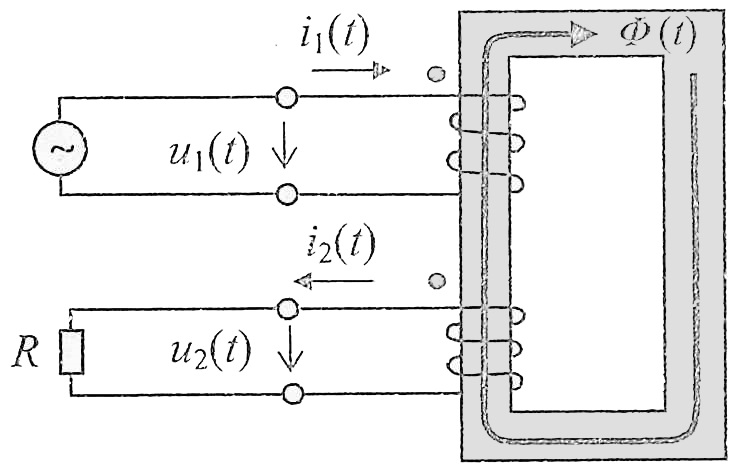
\includegraphics[width=\linewidth]{MJ_patocka_trf.JPG}
      \caption[Princip transformátoru.]{Princip transformátoru. Primární cívka pracuje ve
               spotřebičovém režimu (PPR), sekundární cívka ve zdrojovém režimu (PLR)}
      \label{es:fig_MJ_patocka_trf}
    \end{figure}    
    Z uvedených skutečností lze učinit následující závěr. Volba znaménka v rovnicích
    (\ref{ES:eq_zakl_elm06}a, b) je věcí dohody, ale pouze v tom smyslu, zda zvolíme za základní
    režim spotřebičový či zdrojový\footnote{Ojediněle se v literatuře, např. v [5], vyskytne názor,
    že znaménko v rovnicích (\ref{ES:eq_zakl_elm06}a, b) je určeno tím, zda je cívka navinuta
    pravotočivě nebo levotočivé. To je chybné tvrzení. Pravotočivost či levotočivost cívky naprosto
    nijak nesouvisí se schopnosti cívky pracovat ve zdrojovém nebo spotřebičovém režimu.}. 
    Například při analýze měničů ve výkonové elektronice je ustáleným zvykem zvolit označení proudu
    a napětí na indukčnosti podle obr. \ref{es:fig_MJ_patocka_spbzdr}b. Bez ohledu na tuto volbu
    musíme v konkrétní situaci vždy pečlivě rozlišovat, ve kterém režimu se cívka skutečně nachází.
    Příklad: primární cívka transformátoru se nachází vždy ve spotřebičovém režimu, sekundární
    cívka vždy ve zdrojovém režimu. Se zdrojovým či spotřebičovým režimem úzce souvisí \emph{Lenzův
    princip}\footnote{Heinrich Lenz (1804-1865), estonský fyzik, působil na univerzitě v
    Petrohradu. Princip po něm pojmenovaný objevil r. 1833.}. Jedná se o zvláštní případ
    obecnějšího přírodního principu, vyjádřitelného jako „zákon akce a reakce“. V elektromagnetismu
    má zákon následující tvar:

    Lenzův princip: Proud indukovaný v uzavřené vodivé smyčce vyvolá magnetické pole, které působí
    vždy proti původnímu budicímu poli, díky němuž indukovaný proud vznikl.

    Všimněme si, že zmíněná „uzavřená vodivá smyčka“ se nachází \emph{zdrojovém režimu}: je vložena
    do magnetického pole, indukuje se v ní napětí \(u(t)\), které protlačí vodivým obvodem proud
    \(i(t)\). Proud má ve \emph{zdrojovém režimu} takový směr, že působí proti budicímu magnetickému
    poli. Příkladem je již zmíněná sekundární cívka transformátoru podle Obr. /./-*/« nebo uzavřená
    smyčka vířivého proudu ve vnitřním prostoru transformátorového plechu podle Obr. 1.1-5.

    \begin{figure}[ht!]
      \centering
      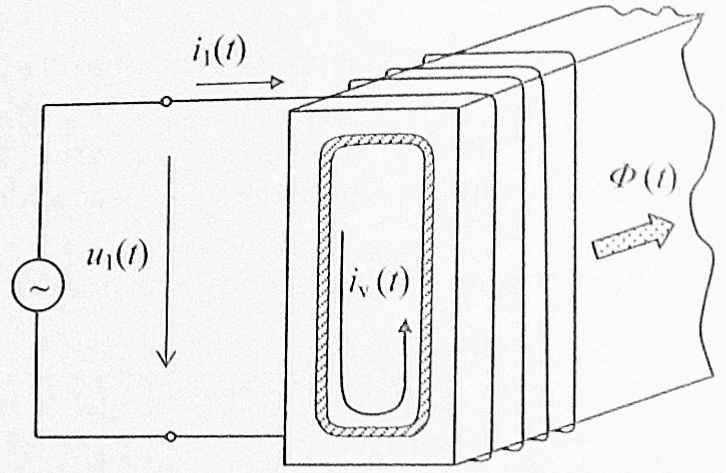
\includegraphics[width=\linewidth]{MJ_patocka_vrvprd.JPG}
      \caption[Vznik vířivého proudu uvnitř elektricky vodivého transformátorového plechu.]{Vznik
               vířivého proudu uvnitř elektricky vodivého transformátorového plechu. Budicí cívka
               pracuje ve spotřebičovém režimu (PPR). Elementární smyčka vířivého proudu odpovídá
          sekundárnímu vinutí a pracuje ve zdrojovém režimu (PLR).}
      \label{es:fig_MJ_patocka_vrvprd}    
    \end{figure}    

    Integrací rovnice (\ref{ES:eq_zakl_elm06}a) lze zpětně dojít k integrálnímu tvaru
    (\ref{ES:eq_zakl_elm05}). Je nutno zdůraznit, že obě rovnice jsou naprosto rovnocenné, navzájem
    převoditelné, obě nesou stejné množství informace, žádná není důležitější než druhá. Je
    pravdou, že z psychologického pohledu je indukční zákon snáze pochopitelný v
    \emph{diferenciálním} tvaru (\ref{ES:eq_zakl_elm06}). Pro hluboké porozumění magnetickým jevům
    je však nezbytné uvědomit si především jeho \emph{integrální} podobu (\ref{ES:eq_zakl_elm05})
    se všemi matematickými důsledky:
    \begin{itemize}
      \item Spřažený tok je roven integrálu napětí. Zákon platí \emph{univerzálně}, bez ohledu na
            \emph{linearitu} či \emph{nelinearitu} magnetického obvodu. Rovnice
            (\ref{ES:eq_zakl_elm05}) totiž definuje funkční závislost \(\Psi=\Psi(u)\) mezi tokem a
            napětím, nikoli závislost \(\Psi=\Psi(i)\) mezi \emph{tokem a proudem}.  Případná
            nelinearita se totiž týká výlučně závislosti \(\Psi=\Psi(i)\), a tudíž nijak nenarušuje
            platnost rovnice (\ref{ES:eq_zakl_elm05}).
      \item Z předchozího bodu plyne, že v obecném \emph{nelineárním} případě není tok \(\Psi\)
            přímo úměrný proudu \(i\). Přímá úměra \(\Psi = Li\) totiž platí pouze ve zvláštním
            případě \emph{lineárního} magnetického obvodu.
      \item Rovnice (\ref{ES:eq_zakl_elm05}) platí ve spotřebičovém i generátorovém režimu cívky.
            Problém se znaménkem zůstává stejný jako u rovnic (\ref{ES:eq_zakl_elm06}).
      \item V uzavřené \emph{supravodivé} smyčce platí vždy \(u = 0\), i když jí teče konstantní
            ss. proud. Neurčitý integrál v rovnici (\ref{ES:eq_zakl_elm05}) má pak nulovou hodnotu
            \(\int0dt=0\), a zřejmě tedy platí \(\Psi(t)=\Psi_0\), kde \(\Psi_0\) je
            \emph{libovolná} počáteční integrační konstanta. Fyzikálně má konstanta význam
            počátečního toku, který je v cívce naintegrován z předchozích dějů. Případ
            \(\Psi_0\neq0\) odpovídá nabuzenému supravodivému magnetu, jehož tok \(\Psi(t)=\Psi_0
            = \text{konst.}\) se s časem nemění. Nabuzený supravodivý magnet se proto chová jako
            \emph{permanentní} magnet. Případ \(\Psi_0 = 0\) odpovídá magnetickému stínění pomocí
            \emph{závitu nakrátko}, např. tzv. Faradayova klec, nebo stínění koaxiálního kabelu
            podle obr. \ref{es:fig_MJ_patocka_koxkbl}. Každé oko \textbf{a-b-c-d} stínícího pláště
            tvoří „supravodivý“ závit nakrátko, v němž platí \(u = 0\), tedy \(\Psi=\int0dt=0\).
            Proto se do vnitřního prostoru ohraničeného pláštěm nemůže zvenčí dostat žádné
            \emph{střídavé} rušivé magnetické pole (jedině pole \emph{stejnosměrné} \(\Psi_{ss}\),
            ale to je neškodné, protože nezpůsobuje vznik rušivého napětí ve středním vodiči
            kabelu; derivace konstanty je totiž nulová: \(u(t)=\frac{d\Psi_{ss}}{dt}=0\)).
    \end{itemize}

    Na otázku „Proč je magnetický tok úměrný integrálu napětí?“ lze odpovědět pouze následujícím
    způsobem: „Protože je to jeden ze základních zákonů přírody, jehož správnost se nepodařilo
    experimentálně nikdy vyvrátit, nýbrž vždy pouze potvrdit.“ Deduktivní odvození indukčního
    zákona z vyšších přírodních zákonitostí není na úrovni klasické fyziky možné, není
    uskutečnitelné ani na vyšší úrovni \emph{kvantové elektrodynamiky}\footnote{Za objev kvantové
    elektrodynamiky obdržel Richard P. Feynman (1918-1988) Nobelovu cenu v r. 1965 (Feynmanovy
    fázorové diagramy a Feynmanův dráhový integrál; nositelé elektromagnetických sil jsou fotony). 
    Vynikající teoretický fyzik, ale i praktik. Celoživotně působil na kalifornském technickém
    institutu. Během druhé světové války byl členem týmu pracujícího na vývoji americké atomové
    bomby v Los Alamos (projekt Manhattan).}. Za povšimnutí stojí, že v diferenciální formě
    (\ref{ES:eq_zakl_elm06}) nebylo přesné kvantitativní ověření indukčního zákona v době objevu
    proveditelné s ohledem na možnosti tehdejšího přístrojového vybavení. Experiment v nehomogenním
    poli podle obr. \ref{es:fig_MJ_patocka_glvnmr} by byl i v současnosti velmi těžko
    vyhodnotitelný. Naopak, ověření v integrálním tvaru je velmi snadné\footnote{V současnosti by
    byl balistický galvanoměr nahrazen operačním zesilovačem zapojeným jako integrační zesilovač.
    Ten by zpracovával signál ze snímače proudu, např. z proudového bočníku. Po odeznění proudového
    impulsu by na výstupu zesilovače zůstalo naintegrováno určité konstantní napětí, jehož velikost
    by analogicky odpovídala maximální výchylce \(\alpha_{max}\) galvanoměru.} . To opravňuje k
    domněnce vyslovené v historickém úvodu kapitoly.
    
    \begin{figure}[ht!]
      \centering
      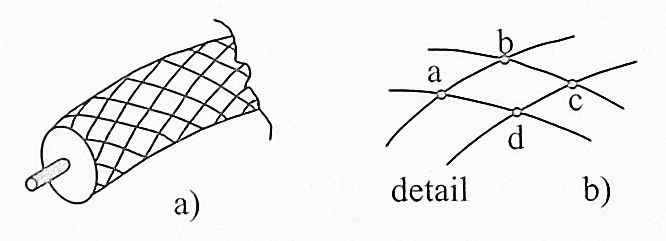
\includegraphics[width=\linewidth]{MJ_patocka_koxkbl.JPG}
      \caption[Plášť koaxiálního kabelu.]{Plášť	koaxiálního kabelu. Každé oko \textbf{a-b-c-d} tvoří
               závit nakrátko.}
      \label{es:fig_MJ_patocka_koxkbl}    
    \end{figure} 
      
    \begin{example}
    Supravodivá cívka podle obr. \ref{es:fig_MJ_patocka_suprvcvk} začne být v okamžiku \(t = 0\)
    napájena ideálním zdrojem napětí \(u(t)\). Později na ni začne působit vnější magnetické pole
    přibližujícího se permanentního magnetu. Jaký vliv bude mít PM na velikost spřaženého toku
    cívky?
    
    Odpověď plyne přímo z rovnice (\ref{ES:eq_zakl_elm05}): \(\Psi(t) = \Psi_0 +\int u(t)dt\).
    \end{example} 
    
    Ze zadání příkladu vyplývá, že počáteční integrační konstanta je nulová. Neurčitý integrál je
    možno nahradit integrálem určitým. Velikost spřaženého toku je tvrdě definována přiloženým
    napětím, tedy hodnotou určitého integrálu. Proto externí magnetické pole nemůže spřažený tok
    cívky nijak změnit. Ideální napěťový zdroj má nulový vnitřní odpor. Proto se supravodivá cívka
    napájená tímto zdrojem stále chová jako supravodivý závit nakrátko, do něhož nemůže vniknout
    žádná siločára externího magnetického pole.
    
    \begin{figure}[ht!]
      \centering
      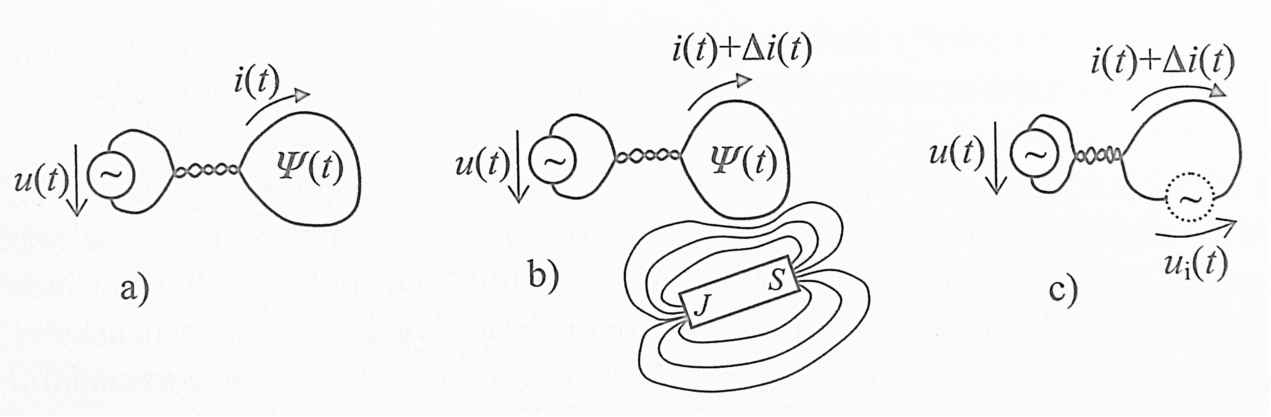
\includegraphics[width=\linewidth]{MJ_patocka_suprvcvk.JPG}
      \caption[Supravodivá cívka]{K příkladu, a) Supravodivá civka je napájená ideálním napěťovým
               zdrojem, b) Později na ni začne působit externí pole pohybujícího se magnetu, c)
               Náhradní zapojení.}
      \label{es:fig_MJ_patocka_suprvcvk}
    \end{figure} 
    
    Jev lze vysvětlit následovně. Pohybující se magnet indukuje v cívce přídavné indukované napětí 
    \(u(t)\). Toto napětí se přičte k napětí napájecímu a způsobí změnu proudu \(\Delta i(t)\)
    tekoucího cívkou. Podle Lenzova principu začne tento přídavný proud působit proti poli PM.
    Přídavný proud \(\Delta i(t)\) má přesně takovou velikost a směr, že uvnitř závitu dokonale
    vykompenzuje a zruší externí pole magnetu. Vnější pozorovatel tedy vidí, že supravodivý závit
    se chová jako magnetický izolant, jemuž se siločáry externího pole vyhnou, a celkový tok cívky
    není přítomností magnetu nijak ovlivněn. Celá soustava se navíc chová jako elektromechanický
    měnič energie (tj. motor), který je schopen pracovat v motorovém nebo generátorovém režimu.
    Pohybující se magnet totiž koná nebo spotřebovává mechanickou práci, protože na něj působí
    síla. Podle vzájemné okamžité orientace vektorů \emph{síly} a \emph{rychlosti} pracuje celá
    soustava buď jako motor (koná mechanickou práci), nebo jako generátor (spotřebovává mechanickou
    energii a ukládá ji do zdroje napětí).
        

    %------------- Spřažený tok vzduchové cívky ----------------------------------------------------
    \section{Spřažený tok vzduchové cívky}\label{es:tokcvk_vzd}
      Experiment s galvanometrem popsaný v předchozí kapitole lze uskutečnit podrobněji ve čtyřech
      následujcících modifikacích označených čísly \textbf{1} až \textbf{4}. Pro vyšší přehlednost
      budou těmito čísly systgematicky značeny i veličiny v jednotlivých pokusech. Ze čtyř postupně
      gradujících experimentů vyplyne geometrická interpretace pojmu \emph{spřažený tok} vzduchové
      cívky. Poznámka: V následujících experimentech se pokusná  cívka nachází v generátorovém
      režimu. Učiníme však dohodu, že velikost toku budeme pro jednoduchost uvažovat v absolutní
      hodnotě, tj. bez ohledu na znaménko \cite[s.~12]{Patocka4}.

      Experiment č. 1:
      Podle Obr ** je na ohebných zkroucených přívodech umístěna tuhá samonosná cívka, která má
      jeden závit o ploše \(\Delta S\). Plocha musí být \emph{malá}, aby bylo možno předpokládat, že
      magnetické pole v těsném okolí cívky je \emph{homogenní} (vektor indukce \(\vr{B_1}\), musí
      být v rámci cívky konstantní). Malé rovinné ploše závitu je pak možno přiřadit vektor
      \(\vr{\Delta S_1}\), jehož směr je kolmý na onu rovinu. Opakováním pokusu při různých úhlech
      \(\alpha_1\), různě velkých plochách a různě velké indukci lze snadno zjistit, že velikost
      toku je přímo úměrná:
      \begin{itemize}
        \item veličině \(\cos\alpha_1\),
        \item ploše závitu \(\Delta S_1 \equiv \Delta S\),
        \item magnetické indukce \(B_1\).
      \end{itemize}
      To vede k jednoznačnému závěru, že tok lze vyjádřit jako skalární součin vektoru plochy a
      vektoru mg. indukce v daném místě „l“:
      \begin{equation}\label{ES:eq_zakl_elm07}
        \int_0^{t_i} u(t)dt = \Psi_1 = B_1\Delta S_1\cos\alpha_1 = \vr{B_1}\cdot\vr{\Delta S_1}.
      \end{equation}  
        
    %------------- Spřažený tok cívky s feromagnetickým jádrem -------------------------------------
    \section{Spřažený tok cívky s feromagnetickým jádrem}\label{es:tokcvk_frmj}
      Principiálně není transformátor nic jiného než soustava vzájemně magneticky vá\-za\-ných
      cívek. Pro jednoduchost je v dalším popisu uvažován transformátor s jedním pri\-már\-ním a
      jedním sekundárním vinutím, přičemž všechny závěry bude možné později rozšířit i na
      složitější systémy. Při odvozování matematického modelu transformátoru vy\-jde\-me z
      Faradayova zákona elektromagnetické indukce (druhá Maxwellova rovnice), který říká, že časová
      změna magnetického pole vytvoří vírové pole elektrické:
      \begin{equation}\label{es:eq_elmag_ind}
        \oint_l \vr{E} \cdot d\vr{l} = - \frac{d}{dt}\int\vr{B}\cdot d\vr{S} =- \frac{d\Psi}{dt}
      \end{equation}
      Vztah platí, uvažujeme-li nulovou velikost posuvného proudu tj. polarizačního a Maxwellova
      proudu. Tvoří-li smyčku $l$ tenký vodič, indukuje se v něm napětí:
      \begin{equation}\label{es_ind_u}
        u(t) = \frac{d\Psi(t)}{dt}
      \end{equation}
      V rov. \ref{es_ind_u} je úmyslně vynecháno záporné znaménko na pravé straně rovnice. To
      platí, je-li na vodič (cívku) pohlíženo jako na spotřebič napájený ze zdroje napětí (což
      odpovídá funkci primárního vinutí transformátoru). Takováto cívka vytvoří časově proměnné
      magnetické pole:
      \begin{equation}\label{es:eq_tok1}
        \Psi(t) = \Psi_0 + \int u(t)dt
      \end{equation}
      Konstanta $\Psi_0$ představuje Newtonovou počáteční integrační konstantu, fun\-kce $\Psi(t)$
      tzv. \textbf{spřažený magnetický tok s cívkou}. Je vidět, že \emph{velikost spřa\-že\-ného
      magnetického toku je úměrná pouze velikosti integrálu napětí na cívce, nemusí již být přímo
      úměrná proudu cívkou} (to platí jen ve speciálním případě lineárních magnetických obvodů).
      Tento poznatek je velice důležitý, magnetický tok bude stejný jak pro vzduchové cívky, tak
      pro cívky s feromagnetickým jádrem (rozdíl bude spočívat pouze v průběhu a velikosti proudu
      cívkou). Sycení jádra transformátoru napájeného ze zdroje napětí je závislé pouze na průběhu
      tohoto napětí. Pro spřažený magnetický tok cívky dále platí:
      \begin{equation}\label{es:eq_tok_indukce}
        \Psi(t) = \oint_S\vr{B}(t)\cdot d\vr{S}
      \end{equation}
      kde $S$ je orientovaná ohraničená plocha, jejíž hranice je tvořena křivkou $l$, viz
      probíhající osou vodiče po celé jeho délce. Tento vztah platí zcela obecně pro jakákoli
      prostředí, v nichž se magnetické pole nachází a pro libovolné tvary plochy $S$. Při návrhu
      transformátoru obvykle známe průběh spřaženého magnetického toku.
      \begin{figure}[ht!]
        \centering
        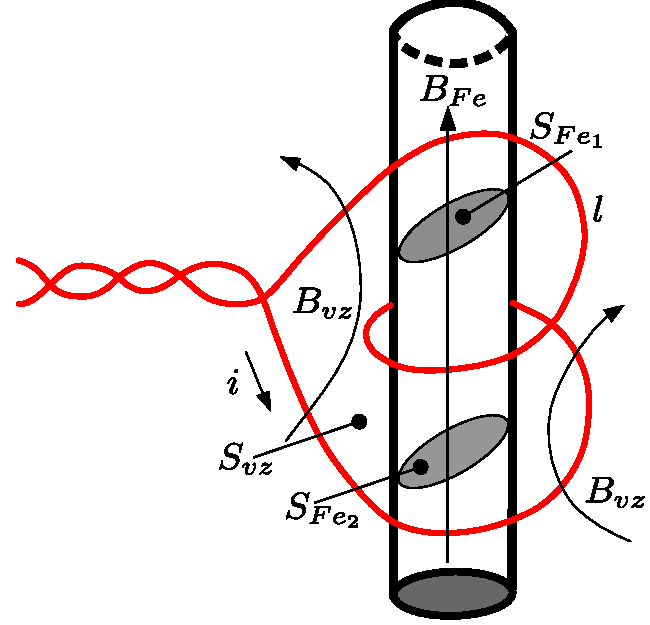
\includegraphics[width=0.8\linewidth]{mag_cir.pdf}
        \caption{Část magnetického obvodu se dvěma závity primárního vinutí.}
        \label{es:fig_Bzv}
      \end{figure}
      Je vidět, že některé indukční čáry $B_{vz}$ neprocházejí materiálem jádra, jedná se o tzv.
      \textbf{rozptyl}. Přesný průběh spřaženého magnetického toku bychom získali aplikací rov.
      \ref{es:eq_tok_indukce}, který bychom pro tento konkrétní případ mohli upravit do podoby
      \begin{equation}\label{es:eq_tok2}
        \Psi(t) = \int \vr{B}_{vz}(t)\cdot d\vr{S}_{vz} + \sum_{i=1}^{N}\int \vr{B}_{Fe}(t)\cdot
        d\vr{S}_{Fe_i}
      \end{equation}
      Protože vyčíslení tohoto vztahu je velice obtížné, zavedeme určité zjednodušující podmínky:
      \begin{itemize}
        \item zanedbáme rozptyl $B_{Fe} \gg B_{vz}$,
        \item magnetická indukce $B_{Fe}$ je ve feromagnetiku rozložena homogenně a siločáry jsou
              kolmé k průřezu jádra.
      \end{itemize}
      Pak pro spřažený magnetický tok můžeme psát
      \begin{equation}\label{es:eq_tok_zjednodus}
        \Psi(t) = N\cdot B_{Fe}(t)\cdot S_{Fe} = N \cdot \Phi(t)
      \end{equation}
      Rov. \ref{es:eq_tok_zjednodus} by platila přesně, pokud by všechny indukční čáry $\vr{B}$
      protnuly plochu $S_{Fe}$ N-krát. Ve skutečnosti ale všechny siločáry neprochází všemi závity a
      vztah platí jen přibližně. Chyba je malá u feromagnetických obvodů (transformátory, cívky s
      feromagnetickým jádrem), kde je magnetická vodivost materiálu mnohonásobně větší, než
      magnetická vodivost vzduchu (řádově 1000x) a rozptyl je tudíž zanedbatelný. Velká je tato
      chyba například u vzduchových cívek, kde je  rov. \ref{es:eq_tok_zjednodus} nepoužitelná.
            
      \begin{equation}
        \begin{array}{rclclcl} 
          \Psi & \cong & N\Phi   & \qquad \text{resp.}  & \qquad \Psi(t)& \cong & N\Phi(t),    \\ 
          \Phi & = & B_{Fe}S_{Fe}& \qquad \text{resp.}  & \qquad \Phi(t)& = & B_{Fe}(t)S_{Fe}.
        \end{array}
      \end{equation}
      
      V literatuře bývá někdy spřažený tok cívky $\Psi$ bez vysvětlení definován pomocí rovnice. To
      je nutno považovat za nešťastné. Za prvé se nejedná o "definici'', ale o výsledek značně
      složitých výpočtů, za druhé tato rovnice \emph{principiálně není přesná}

\printbibliography[heading=subbibliography]